\documentclass[11pt]{article}
\usepackage{lineno, graphicx, setspace, amsmath, csvsimple, booktabs}
\usepackage[numbib, nottoc]{tocbibind}
\usepackage[font=footnotesize, labelfont=bf]{caption}

\linenumbers
\setstretch{1.5}
\setlength{\topmargin}{-2cm}
\setlength{\oddsidemargin}{0cm}
\setlength{\textheight}{24cm}
\setlength{\textwidth}{16cm}

\newcommand\wordcount{\input{wordcount.txt}}


\title{\textbf \huge Holling's disc equation outperforms quadratic and cubic linear models regarless of AIC cut-off threshold} 
\author{ \large Amisha Bhojwani \\ \small MSc Computational Methods in Ecology and Evolution \\ \small Imperial College London 2020-21 \\}
\date{ \small 22nd January, 2021}

\begin{document}
  
  \begin{titlepage}
    \centering
    \maketitle
    \normalsize
    Wordcount: \wordcount{}
  \end{titlepage}
  
  \tableofcontents{}
  \pagebreak
  
  \abstract
  A functional response describes the relationship between consumer predation rate and resource density \cite{Solomon1949}. Holling’s disc equation, also known as the Type II functional response, is the most frequent type of functional response model in the literature \cite{Jeschke2002}. In this study I analyse how well it describes a dataset with a variety of species interactions between taxa and expect it to do so at a higher rate than a phenomenological approach to modelling. Additionally, I investigate the differences in results when considering different Akaike Information Criterion (AICc) cut-off values for establishing a confidence set of models. I found that using Schwarz Criterion and $R^2$ values skewed my results as these don’t account for small sample sizes, unlike AICc. By considering AICc values I find that the disc equation is indeed the chosen most parsimonious model at a higher rate than the linear quadratic and cubic phenomenological models, regardless of cut-off values.
  
  \section{Introduction}
  
  A functional response is the relationship between consumer predation rate and prey density \cite{Solomon1949}. Holling (1959) \cite{Holling1959} described three functional response models which stem from scenarios that he termed “artificial situations”. From these controlled experiments he gathered that there are two behaviours present in all predator-prey situations; time spent searching for prey ($a$) and the time spent handling prey ($h$). These insights led to him defining a general functional response equation:
  
  \begin{linenomath*}
    \begin{equation}
      y=\frac{ax}{1+ahx}\label{eq:1}
    \end{equation}
  \end{linenomath*}
  
  Where $y$ is consumption rate (resources consumed per time unit and predator) and $x$ is prey density (number of individuals per unit of area or volume). It is important to note that Hollings search rate ($a$) implies a $100\%$ success rate  and is often also referred to as such \cite{Holling1959}. The above equation can also be referred to as Holling’s disc equation or, what he later defined as, a Type II functional response equation. The curve from this equation presents a negatively accelerated rise to a plateau, unlike the Type I functional response which he describes as a linear rise to a plateau. A Type III functional response is also described, and it accounts for another parameter, according to Holling it is a learning component, that results in an S-shaped curve. 
  
  Holling (1959) \cite{Holling1959} denotes that the disc equation is general and malleable enough to accommodate interaction specific parameters which may help further explain biological data. Aljetlawi (2004) \cite{Aljetlawi2004} emphasises this by explaining how the components of an interaction vary between and within species not only on an individual level but also at community level, meaning that the terms $a$ and $h$ in the disc equation may have interaction-specific biological meanings and could encompass more than one mechanism.
  
  The artificial predation systems used to derive Holling’s disc equation do not reflect natural ones and the model is therefore considered to be unrealistic by some \cite{Jeschke2002}. To overcome this, we must consider that there are factors which can interfere and influence the biological meaning Holling attributed to his parameters $a$ and $h$ which can be used to explain biological data in more detail \cite{Aljetlawi2004}. For example, digesting is different from handling but may influence a predator's reason behind searching for new prey. The extensions to the original disc equation made in Holling's 1966 publication \cite{Holling1966} are the only ones to treat digestion as a factor of influence to foraging activity due to its relationship with prey density; prey density will determine satiation levels which will, in turn, drive a predator’s search rate. Furthermore, in the disc equation, eating time is modelled together with handling time \cite{Jeschke2002}, so more detail is required in describing the biological mechanisms that a single parameter represents, as the mathematical relationship with other parameters may change as a consequence. These considerations point towards the need of fine-tuning the disc equation to the specificity desired in an interaction and incorporating parameters, such as satiation, to further expand the biological meaning the model can provide. 
  
  Foraging theory is not the only theoretical framework to be considered among the literature for functional response models; mechanistic models proposed vary in form and nature and tend to branch out from the disc equation. A family tree of functional response models is available in the literature \cite{Jeschke2002}, and from it we note the possibility to modulate between models. For example, the disc equation can be modified to include a parameter q that helps modulate from a Type II to a Type III response \cite{Real1977,Real1979}:
  
  \begin{linenomath*}
    \begin{equation}
      y=\frac{ax^{1+q}}{1+ahx^{1+q}}\label{eq:2}
    \end{equation}
  \end{linenomath*}
  
  The value $q=1$ would mean the equation takes the form of Holling’s Type III functional response, whereas at $q=0$ it equates to a Type II functional response. Jeschke (2002) \cite{Jeschke2002} argues that this equation should be considered phenomenological as it doesn’t explain the mechanisms at play in a Type III response, particularly, that the added parameter ($q$) is not explained mechanistically as needed. 
  
  In this study I analyse how well the disc equation \eqref{eq:1} can describe data from a multiplicity and variety of species interactions in a large dataset, and compare it to two phenomenological approaches. I use the equation from \eqref{eq:1} and do not consider the approach in \eqref{eq:2} in order to avoid mixing mechanistic and phenomenological approaches within the same model. The interactions in the studied dataset range from vertebrates, to invertebrates to plants and encompass both terrestrial and aquatic environments, attributing it a wide range of taxa to work on. I do not consider the Holling Type III model in this study because, if the Type II functional response is the most observed in the literature \cite{Jeschke2002}, I expect that the mechanistic Holling Type II model will describe a high percentage of our data, moreover, it will do so more appropriately than a phenomenological approach would allow. 
  
  I will also investigate if the final confidence set of models for the data would differ depending on the cut-off values used to declare it, as there is discussion that the general rule of $\Delta_{AIC}\leq2$, where the models in the confidence set have to be less than two units away in AIC from the model with the minimum AIC, is too restrictive and might avoid including the truly most parsimonious model in the confidence set \cite{Richards2008, Richards2011}.

  \section{Methods}
    \subsection{Data analysis}
    
    The dataset considered was collected from lab and field experiments worldwide and holds the rates of prey consumption by consumers from a variety of species interactions. There's over 50 fields of metadata for this dataset but for the purposes of this report I used fields containing the number of resources consumed per predator per unit time and the resource density, the latter of which varied in units depending on the dimensionality of the interaction studied. The dataset has 308 individually identified interactions (ID’s) and each one has at least 4 observations, 142 being the most observations for one interaction. Overall, almost 70\% of the subsets have a sample size of less than 10. We must note that there might be more than one ID with observations for a particular species interaction, this may be because the data comes from different sources and may represent the interaction in different contexts (laboratory or field settings). Also noteworthy is the existence of replicates in the data, which affect the fitted models as we see in Fig. \ref{fig:egplots}.
    
    I subset the data by individual interactions and fit three models to each subset: a quadratic linear model, a cubic linear model and the Holling Type II functional response model \cite{Holling1959}. The two first models are phenomenological and I fit them using Ordinary Least-Squares (OLS) methods whilst the last is mechanistic and I used Levenberg–Marquardt Non-Linear Least-Squares (NLLS-LM) methods to fit it.  
    
    The Type II model works with two parameters, as seen in equation \eqref{eq:1}, and I estimated them using parametrizations before modelling. The parameter $h$ is the inverse of the maximum feeding rate ($h=1/F_{max}$) and the parameter $a$ is the maximum feeding rate divided by the prey density at which the predator consumes half the amount of its feeding rate ($a=F_{max}/N_{Half}$) \cite{Real1977, Rosenbaum2018}. The parameter estimations were then sampled from a uniform distribution around the estimated values to further improve their approximation to the data. We bound the parameters at 0 for this to be their lowest possible value, as we know there will never be negative attack rates or handling times.
    
    To compare the three competing models, as well as select the sampled parameters, I used model selection criteria because it considers not just how well the model fits the data but also how complex the model is. Furthermore, this criteria allows us to compare more than two models simultaneously, differentiating this method from null hypothesis significant testing (NHST). To compare only the fit of the models, I extracted $R^2$ values from each model fit \cite{JohnsonOmland2004}.
    
    I calculated Akaike’s Information Criterion (AIC) derived for small sample sizes (AICc) by Sugiura (1978) and Hurvich and Tsai (1989) \cite{Burnham2011}. I also calculated Schwartz Criterion for the purposes of model selection. AIC measures the amount of Kullback-Leibler (KL) information loss, accounting for lack of fit, bias correction and model complexity. Schwartz Criterion is also known as the Bayesian Information Criterion (BIC) and is superficially similar to AIC except it includes an expression for sample size dependency and is not based on KL information theory. I used AICc for model selection rather than AIC because the number of parameters used in each model exceeded $n/40$, where $n$ is sample size, so AICc allows me to account for the smaller sample sizes of the subsets of data \cite{JohnsonOmland2004}. Furthermore, AICc converges to AIC when sample sizes are large so to use it could avoid errors if one hasn't accounted for sample sizes \cite{Burnham2011}.

    Model selection with model selection criteria such as AIC can work with cut-off values to identify a confidence set of models among which the most parsimonious model will be $95\%$ of the time. Generally, it is considered that if a model has a difference in AIC value less than than 2 from the model with the smallest AIC value ($\Delta\leq2$), it falls within the confidence set of models \cite{BurnhamKennethP2002}. However, Richards (2011) argues that this consideration is too restrictive and may elude the truly most parsimonious model from the confidence set. Simulations show that for the truly most parsimonious model, according to the data, to be in the confidence set, it should be that $\Delta\leq6$ \cite{Richards2011}. For this study, I considered both these approaches alongside a no-cut-off approach, where the model with the lowest AIC is the most parsimonious in the a priori set of models.
      
    \subsection{Computing tools}
    For the entirety of the data analysis part of this project I used R version 4.0.3. R language makes modelling possible in very few lines of code with user friendly and intuitive syntax. The RStudio IDE allows for easy, quick and readily visual data exploration. I point out the visual exploration because of the integrated graphics device and because packages such as \emph{ggplot2} make quick plotting very accessible. R also boasts of a rich packages library for statistics, one of which I used for this project: \emph{minpack.lm}. I wanted to keep the dependencies on this project relatively minimal so I havent used any other packages aside from the ones I've mentioned here on R. For writing this report I've used Latex, pdfTeX version 3.14159265-2.6-1.40.20 (TeX Live 2019/Debian), because it's useful to format reports that include figures and data that update in real time. It also has a convenient reference management method, \emph{BibTeX}. Packages I've used to write this report include:

    \begin{itemize}
      \item[--] \emph{graphicx} to include graphics in the report
      \item[--] \emph{setspace} to indicate text spacing and margins of the document
      \item[--] \emph{lineno} to enumerate each line
      \item[--] \emph{amsmath} for writing equations, referencing them and writing in-line maths
      \item[--] \emph{csvsimple} allows importing of csv files to produce Latex tabulars
      \item[--] \emph{booktabs} allowed me to format tables
      \item[--] \emph{tocbibind} allowed the References section to be numbered and therefore appear in the table of contents 
    \end{itemize}

    To count the words in the report I used a script in Perl version v5.30.0 called \emph{texcount}. The last computing tool I used is Bash, GNU bash version 5.0.17(1), to write a shell script that compiles the entire project. I chose Bash over Python because the syntax is succint and is how I would run the project from a terminal.
  
  \section{Results}
  
  Surprisingly, the phenomenologic cubic model seems to fit the data better than the mechanistic model chosen, as evidenced by the higher proportion of times when it's chosen according to the $R^2$ values in Table \ref{table:RsqBIC}. The model fits are best for the cubic model in subsets with the lowest sample size ($n=4$), where the model is able to fit the data perfectly ($R^2=1$) and the AIC and BIC values are $-Inf$ (panel two in Fig. \ref{fig:egplots}).

  \begin{table}[h]
    \centering
    \small
    \csvautobooktabular{../Results/output_tables/Rsq_BIC_table.csv}
    \caption{Proportion of times the model is chosen as: the model with the best fit (highest $R^2$) or the most parsimonious model (lowest BIC).}
    \label{table:RsqBIC}
  \end{table}

  Even though the quadratic model never has the highest $R^2$ among all three models for one subset of data, the values tend to be high: $R^2>0.90$ for $\sim80\%$ of the subsets. The remaining models then manage to have a perceptibly higher fit for most subsets of data. Despite not having the best fit of the three, the quadratic model presents the lowest BIC, deeming it the most parsimonious model of the three according to this criterion. The support for the cubic and Holling Type II models does not differ much, both being chosen at a rate of 0.4 when considering BIC (Table \ref{table:RsqBIC}).
  
  \begin{table}[h]
    \centering
    \small
    \csvautobooktabular{../Results/output_tables/AIC_table.csv}
    \caption{Proportion of times that when said model has the lowest AICc value for a subset, it is the only one in final set of confidence models. Conversely, the inverse of the rates represented indicate that there are at least two models in the confidence set. When there is no cut-off, the model that has the lowest AIC is considered the only one in the confidence set. The "Overall" fields are irrespective of the model type, for example overall, when there is no cut-off, there is one most parsimonious model per subset of data all of the time. An example on how to read the table would be as follows: the quadratic model has the lowest AIC value $\sim15\%$ of the time, if we consider a cut-off at 2 approach ($\Delta\leq2$), the quadratic model will be the most parsimonious model, standing alone in the confidence set, $\sim5\%$ of the time. In contrast, if the cut-off is $\Delta\leq6$, it will rarely remain alone in the confidence set ($\sim1\%$ of the time).}
    \label{table:AIC}
  \end{table}

  In terms of AIC, a general trend we see is that a lower cut-off translates to considering only one model in the confidence set $\sim80\%$ of the time, whereas with a higher cutoff this value is lessened to $\sim50\%$. If we are considering the former, that cut-off values are $\Delta\leq2$, the Holling Type II model remains the only model in the confidence set $\sim85\%$ of the times that it is the model with the lowest AIC for a subset. Furthermore, when contrasted with the other models, and regardless of the cut-off type, Holling's Type II model is consistently chosen as the most parsimonious model for the data at higher rates than the cubic and quadratic models (Table \ref{table:AIC}).
  
  \begin{figure}[h]
    \centering
    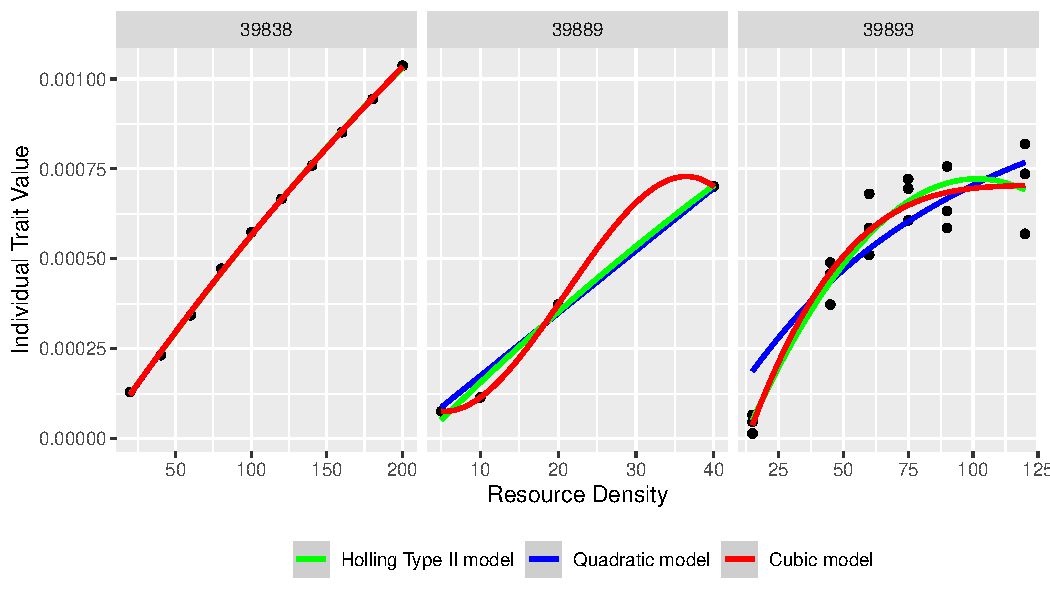
\includegraphics[scale=0.8]{../Results/output_tables/plots.pdf}
    \caption{Plots showing the fit of all three models in the a priori model set for three ID numbers. The interaction in ID number 39838 is between \emph{Rhyacophila dorsalis} (consumer) and \emph{Chironomus spp} (resource). The interaction in ID number 39889 is between \emph{Plectrocnemia conspersa} (consumer) and \emph{Nemurella picteti} (resource). The interaction in ID number 39893 is between \emph{Peromyscus maniculatus} (consumer) and \emph{Triticum spp.} (resource).}
    \label{fig:egplots}
  \end{figure}

  Visual representations of the different fits can be found in the "Results" directory of this project under a subdirectory named "plots". In this paper we include three examples. Firstly, we see times where the fits of all three models are almost indistinguishable (panel 1 Fig. \ref{fig:egplots}). Secondly, the cases where AIC and BIC values for the cubic model were $-Inf$ happens in subsets like the one in panel 2 of Fig. \ref{fig:egplots}, where the sample size was small ($n=4$). Lastly, an example of a subset having replicates for select values of resource densities can be seen in the last panel of Fig. \ref{fig:egplots}.
  
  \section{Discussion}
  
  This study analyses how well the disc equation can fit a dataset in comparison to two phenomenological models and how a final set of confidence models is affected by AIC cut-off values. From our analyses we can say that the Holling Type II model receives the most support when considering AIC values but the quadratic model receives the most support when considering BIC. Both AIC and BIC are able to incorporate fit and model complexity in their index \cite{JohnsonOmland2004}, so there must be a reason for the disagreement between both selection criteria.

  Over 70\% of the subsets of data have 10 or less observations. The subsets are generally too small for BIC to be reliable for model selection because, for this index, the "true model" is identified with maximum probability as the sample size increases to infitinity (Schwarz 1978 cited in \cite{Burnham2011}). Another BIC caveat is the notion that the true model is in the a priori set of models under consideration, if this is not the case the criterion is inconsistent \cite{Burnham2011}. We did not include interaction specific models in the initial set of models, so it may well be that for certain subsets BIC is unreliable because the true model was in fact not considered in the initial set of models.

  The mistaken analysis of small sample sizes did not only affect the consideration of BIC indexes and appropriate model selection criteria, it also led to overfitting of the cubic model to the data as seen in the second panel of Fig. \ref{fig:egplots}. This would explain why the cubic model is consistently chosen as the model of best fit $\sim90\%$ of the time.

  These mistakes in model inferencing can be palliated by looking at our AICc values. When we computed AICc values we accounted for small sample sizes. We also know that AIC indexes work with KL Information Theory (IT) and tell us about the amount of real information lost to the model \cite{JohnsonOmland2004}. In this way, the assumption that the true model is in the a priori model set is avoided. Furthermore, AIC looks to maximise fit and minimise information loss, criteria that are attractive for multi-model inferencing.

  Now only considering our AICc values, we can say that higher cuto-ffs lead to considering more than one model in a confidence set. In the case of this study, if there is only one chosen model after model selection, it is the mechanistic Holling Type II model at a rate of 0.65 when considering $\Delta\leq2$, and at a rate of 0.44 when considering $\Delta\leq6$, always at least a 0.35 rate higher than the remaining models. This would mean that the Holling Type II model is the most parsimonious among the ones considered at a higher rate than the quadratic and cubic linear models, a finding consistent with our initial hypothesis and with the number of times it has the lowest AICc value without considering a cut-off (Table \ref{table:AIC}). In terms of AICc cut-off values they don't tend to affect the higher rate of selection of the Holling Type II model from among the a priori set of models, but they do decrease the number of times it is considered the lone standing most parsimonious model in a confidence set the higher the cut-off is.

  \bibliographystyle{plain}
  \bibliography{report}
\end{document}